% !TeX encoding = UTF-8
% !TeX spellcheck = pl_PL
\chapter{Badanie efektywności}
Badanie efektywności odbyło się dwojako. Przy użyciu symulacji numerycznej w programie Matlab, jak i poprzez eksperymenty w terenie.
\section{Symulacja numeryczna}
Wszystkie kody symulacji wykorzystane w pracy znajdują się w dodatku C.
Na poniższej grafice widać jak propaguje się sygnał na ścieżce wolnej, interesuje nas w szczególności część wykresu dla częstotliwości w okolicach 1 GHz, czyli takiej jaką wykorzystuje protokół Lora.
\includegraphics*{./grafika/num_sim1_straty_na_sciezce.png}

W rzeczywistości jednak sygnały nie poruszają się w próżni, więc straty na ścieżce wolnej opisują tylko część tłumienia sygnału.
Sygnały interferują z cząsteczkami w powietrzu i tracą energię na drodze propagacji. Straty różnią się w zaleźności od różnych czynników takich jak: ciśniecie, temperatura, opad atmosferyczny, rodzaj i gęstość opadu, zachmurzenie lub jego brak.

Poniżej znajduje się wykres przedstawiający tłumienie podczas opadu deszczu, na dystansie 5 km. Interesuje nas w szczególności część wykresu na jego początku, właśnie w takim zakresie częstotliwości, w jakim działa Lora.
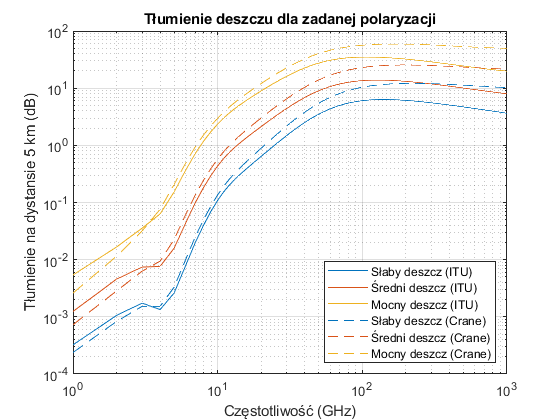
\includegraphics{./grafika/num_sim2_tlumienie_podczas_opadu_deszczu.png}

Ponownie, poniżej wykresy, tym razem podczas opadu atmosferycznego w postaci śniegu, w 3 stopniach nasilenia, dla 2-óch odległości.
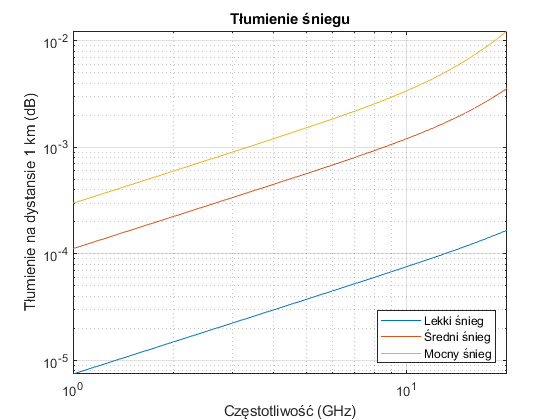
\includegraphics{./grafika/num_sim3_tlumienie_podczas_opadu_sniegu_1km.png}
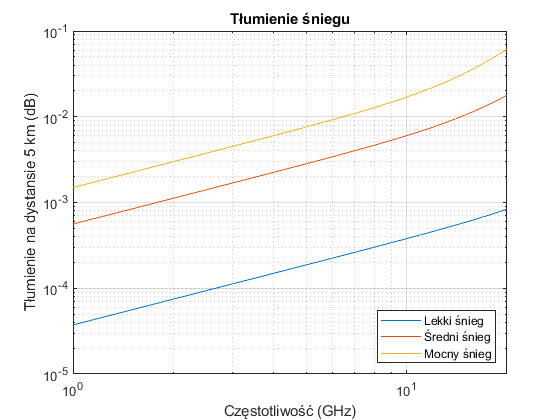
\includegraphics{./grafika/num_sim4_tlumienie_podczas_opadu_sniegu_5km.png}
\pagebreak
\section{Badanie terenowe}\cite{pico2024}